\section{scrum flow}

\subsection*{sprints}

All work is done in Sprints, each Sprint is an iteration of 30 consecutive calendar days.

Each Sprint is initiated with a Sprint planning meeting, where the Product Owner and Team get together to collaborate about what will be done for the next Sprint.

Selecting from the highest priority Product Backlog, the Product Owner tells the Team what is desired.



\subsection*{sprint planning}

Sprint meeting should not last longer than 8 hours.

The Sprint planning meeting has two parts: 

\begin{itemize}
  \item first four hours
  \begin{itemize}
    \item are spent with the Product Owner presenting the highest priority Product Backlog to the Team
    \item The Team questions him or her about the content, purpose, meaning, and intentions of the Product Backlog
    \item When the Team knows enough, selects as much Product Backlog as it believes it can turn into a completed increment of potentially shippable product functionality by the end of the Sprint.
  \end{itemize}
  \item second four hours
  \begin{itemize}
    \item the Team plans out the Sprint
    \item The tasks that compose this plan are placed in a Sprint Backlog
    \item the tasks in the Sprint Backlog emerge as the Sprint evolves
  \end{itemize}
\end{itemize}

directly after the meeting, the sprint has started, 30 day target is tried to be met.



\subsection*{daily scrum}

Every day, the team gets together for a 15-minute meeting called a Daily Scrum.

each Team member answers three questions:

\begin{itemize}
  \item What have you done since last Daily Scrum?
  \item What do you plan on doing between now and next Daily Scrum?
  \item What impediments stand in the way of you meeting your commitments to this Sprint and this project? 
\end{itemize}

purpose of the meeting is to
\begin{itemize}
  \item synchronize each team member daily
  \item to schedule any meetings that the Team needs to forward its progress
  \item keeps all team activities visible so that the ScrumMaster can enforce the rules and help the team stay on track.
\end{itemize}



\subsection*{review meeting}

At the end of the Sprint a Sprint review meeting is held, it is an informal meeting.

four-hour meeting at which the Team presents what was developed during the Sprint to the Product Owner and any other stakeholders

purpose of the meeting is to
\begin{itemize}
  \item functionality is presented is intended to bring people together
  \item collaboratively determined what the Team should do next
\end{itemize}


\subsection*{Sprint retrospective}
After the Sprint review and prior to the next Sprint planning meeting, the ScrumMaster holds a Sprint retrospective meeting with the Team. three-hour meeting: revise the Teams development process to make it more effective and enjoyable for the next Sprint. 

\begin{figure}[H]
  \centering
  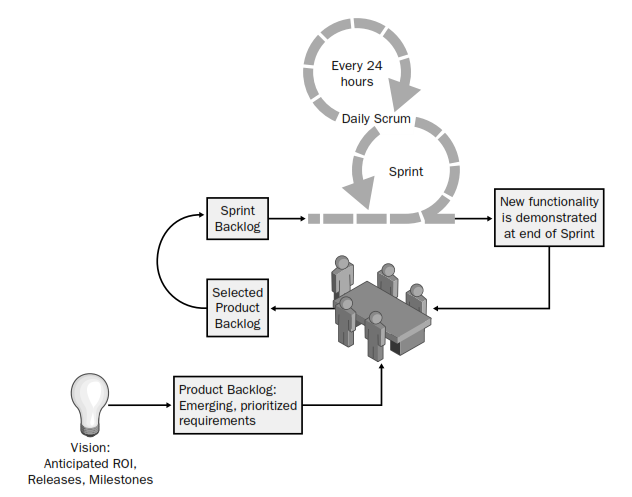
\includegraphics[width=0.6\textwidth]{./figures/chapter_1/scrum_process_overview.PNG}
  \caption{scrum process overview}
  \label{fig:ch1-scrum_process_overview}
\end{figure}\bigskip


